% This file was created with matplot2tikz v0.5.3.
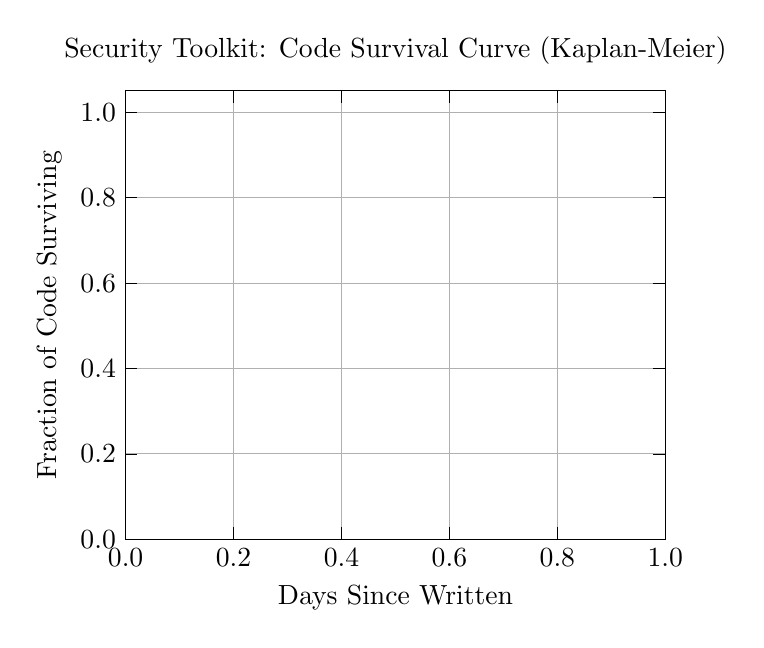
\begin{tikzpicture}

\definecolor{darkgray176}{RGB}{176,176,176}

\begin{axis}[
legend style={fill opacity=0.8, draw opacity=1, text opacity=1, draw=none},
tick pos=both,
title={Security Toolkit: Code Survival Curve (Kaplan-Meier)},
x grid style={darkgray176},
xlabel={Days Since Written},
xmajorgrids,
xmin=0, xmax=1,
xtick style={color=black},
xtick={0,0.2,0.4,0.6,0.8,1},
xticklabels={
  \(\displaystyle {0.0}\),
  \(\displaystyle {0.2}\),
  \(\displaystyle {0.4}\),
  \(\displaystyle {0.6}\),
  \(\displaystyle {0.8}\),
  \(\displaystyle {1.0}\)
},
y grid style={darkgray176},
ylabel={Fraction of Code Surviving},
ymajorgrids,
ymin=0, ymax=1.05,
ytick style={color=black},
ytick={0,0.2,0.4,0.6,0.8,1,1.2},
yticklabels={
  \(\displaystyle {0.0}\),
  \(\displaystyle {0.2}\),
  \(\displaystyle {0.4}\),
  \(\displaystyle {0.6}\),
  \(\displaystyle {0.8}\),
  \(\displaystyle {1.0}\),
  \(\displaystyle {1.2}\)
}
]
\end{axis}

\end{tikzpicture}
